%%%%%%%%%%%%%%%%%%%%%%%%%%%%%%%%%%%%%%%%%
%
% Funkcionalna verifikacija hardvera
% 
%%%%%%%%%%%%%%%%%%%%%%%%%%%%%%%%%%%%%%%%%

Deseta vežba je posvećena \emph{scoreboard}-u. Opisana je podela verfikacionih
okruženja na osnovu načina vršenja provere očekivanih rezultata, opisana je
implementacija \emph{scoreboard}-a prateći UVM i opisane su često korišćene
funkcionalnosti. Takođe je dat primer verifikacionog plana i opisana veza plana
sa proverama u samom okruženju.

%========================================================================================
% Section
%========================================================================================

\section{Podela verifikacionih okruženja}

Jedna od osnovnih podela verifikacionih okruženja odnosi se na način kako se
vrši provera očekivanih rezultata. Prema ovom kriterijumu sva okruženja mogu se
podeliti u dve velike grupe:

\begin{itemize}
\item Okruženja bazirana na konceptu ``zlatnih vektora''
\item Okruženja bazirana na referentnim modelima
\end{itemize}

% ----------------------------------------------------------------------------------------

\subsection{``Zlatni vektori''}

Kod ovog tipa okruženja stimulus koji je neophodno dovesti na ulaze sistema koji
se verifikuje, kao i očekivani odziv na svaki od ovih stimulusa unapred je
definisan i smešten u skup takozvanih ``zlatnih vektora''. Pod zlatnim vektorom
podrazumeva se jedan par vrednosti ulaznih signala sistema koji se verifikuje i
očekivanog izlaza sistema u tom slučaju. Obzirom da su ulazi i izlazi u sistem
zadati u vektorskoj formi (kao niz individualnih vrednosti za svaki od ulaznih
portova i niz očekivanih vrednosti na svakom od izlaznih portova sistema koji se
verifikuje), jedan ovakav par čini jedan ``zlatni vektor''. Za obavljanje
verifikacije nije dovoljan samo jedan zlatni vektor već je neophodan veliki skup
različitih zlatnih vektora. Ovaj skup zlatnih vektora najčešće se smešta u
odgovarajuću datoteku koja se na početku simulacije učitava u verifikaciono
okruženje. Prilikom simulacije testbenč uzima jedan po jedan zlatni vektor iz
skupa i njegovu ulaznu komponentu dovodi na ulaze sistema koji je potrebno
verifikovati. Nakon što se u procesu simulacije izračuna odziv sistema koji se
verifikuje na ovu ulaznu komponentu zlatnog vektor, on se upoređuje sa izlaznom
komponentom tekućeg zlatnog vektora. Ukoliko su oni identični proces
verifikacije se nastavlja sa sledećim zlatnim vektorom. U slučaju da dolazi do
odstupanja, proces verifikacije sa prekida, a identifikovano odstupanje se
saopštava verifikacionom inženjeru kako bi mogao započeti proces lokalizacije
greške (\emph{bug tracing}) unutar sistema.

% ----------------------------------------------------------------------------------------

\subsection{Referenti modeli}

Glavni nedostatak testbenčeva baziranih na ``zlatnim vektorima'' ogleda se u
činjenici da je pre početka procesa potrebno generisati odgovarajući skup
``zlatnih vektora''. Ovaj postupak se često radi ručno, od strane verifikacionog
inženjera, i uključuje ne samo osmišljavanje interesantnih vrednosti ulaznog
stimulusa, već i izračunavanje očekivanog ponašanja sistema koji se verifikuje
na ovakav stimulus. Pošto se često radi ručno, ovaj proces je spor i podložan
greškama koje zatim usporavaju dalji proces verifikacije.\\

Način kako da se ovaj nedostatak pristupa baziranog na ``zlatnim vektorima''
može prevazići je korišćenje testbenčeva baziranih na referentim modelima.\\

Pod referentnim modelom podrazumevamo model sistema koji se verifikuje napisan
na visokom nivou apstrakcije. Referentni model treba da poseduje željenu
funkcionalnost koja je trebalo da bude implementirana unutar sistema koji se
verifikuje. Obzirom da se referentni model piše na visokom nivou apstrakcije on
je znatno jednostavniji od modela sistema koji se verifikuje što olakšava njegov
razvoj i smanjuje mogućnost unošenja nenamernih grešaka prilikom njegovog
pisanja. Referentni model se unutar testbenča koristi kao refernca (otuda i
njegovo ima) koja služi za poređenje odziva dobijenih od strane sistema koji se
verifikuje na dovedenu pobudu.\\


Proces verifikacije unutar testbenča baziranog na referentnom modelu odvija se
na sledeći način. Unutar testbenča instancionirane su dve komponente: model
sistema koji želimo da verifikujemo i njegov referentni model. Prilikom procesa
simulacije na ulaze oba modela dovode se iste sekvence ulaznih vektora, a odzivi
referentnog modela i modela sistema koji se verifikuje se zatim porede kako bi
se utvrdilo da li postoji neko odstupanje. Obzirom da oba modela modeluju istu
funkcionalnost odstupanja ne bi trebalo da bude. Ukoliko se da je do odstupanja
došlo, to predstavlja indikaciju o postojanju greške unutar nekog od dva modela.
Simulacija se u tom trenutku prekida, a zadatak verifikacionog inženjera je da
utvrdi u kojem od modela se nalazi greška.\\

Svi referentni modeli mogu se podeliti u dve velike grupe, prema tome koliko
precizno modeluju funkcionalnost koju sistem koji se verifikuje treba da
poseduje:

\begin{itemize}
\item Transakcione referentne modele (``transaction level'' referentni modeli -
  ovi referentni modeli modeluju očekivano ponašanje sistema koji se verifikuje
  do nivoa transakcija, a ne individualnih perioda (ciklusa) klok signala.
  Transkcija predstavlja apstrakciju procesa obrade podataka unutar nekog
  sistema, pri čemu se vremenski period potreban za završetak obrade zanemaruje.
  Jedino što nas kod transakcija interesuje jeste rezultat obrade nekog ulaznog
  podataka (šta god ta obrada podrazumevala), a ne i vremenski redosled koraka
  koji dovodi do tog rezultata.
\item Referentne modele na nivou ciklusa (``cycle accurate'' referentni modeli
  - ovi modeli, za razliku od transakcionih, modeluju očekivano ponašanje
  sistema koji se verifikuje sve do nivoa individulanih ciklusa klok signala.
\end{itemize}

Zbog svih prethodno navedenih osobina, u praksi se često sreće transakcioni
referentni model. I u UVM metodologiji se koristi ovaj model koji je uglavnom
impementiran u sklopu \emph{scoreboard}-a. U literaturi se sreće i naziv
\emph{predictor}.

%========================================================================================
% Section
%========================================================================================

\section{\emph{Scoreboard}}

Važan element svakog \emph{self-checking} okruženja je upravo \emph{scoreboard}.
U njemu se uglavnom vrše provere ispravne funkcionalnosti sistema koji se
verifikuje na sistemskom nivou. Sadržaj i uloga \emph{scoreboard}-a dosta zavisi
od same implementacije, ali u većini slučajeva je povezan sa ostatkom okruženja
preko TLM interfejsa preko kojih prima transakcije. Te transakcije zatim
analizira uz pomoć referentnog modela ili zlatnih vektora i poredi očekivane
rezultate sa dobijenim transakcijama. Referentni model može biti implementiran u
sklopu samog \emph{scoreboard}-a ili kao zasebna komponenta.\\

\emph{Scoreboard} se nalazi u UVM \emph{environment} klasi odakle
može komunicirati sa monitorima ili ostalim komponentama.
\emph{Scoreboard} nije povezan sa DUT-om jer sve potrebne informacije treba da
dobija iz odgovarajućih monitora, a ne direktno preko interfejsa.

% ----------------------------------------------------------------------------------------

\subsection{Uloga}

\emph{Scoreboard} je često najkompleksniji deo okruženja i najteži za
implementaciju. Može se podeliti na dva glavna dela: predikcija i evaluacija.
Prvi korak je utvrditi šta je ispravna funkcionalnost odnosno koji rezultat
očekujemo. Kada se tačan rezultat utvrdi vrši se provera rezultata DUT-a odnosno
da li se observirani rezultati slažu sa očekivanim. Dobra praksa je razdvojiti
ova dva glavna zadatka \emph{scoreboard}-a. Time se dobija na fleksibilnosti
koda i olakšava se ponovna upotreba.\\

\begin{figure}[h!]
  \center
  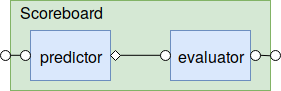
\includegraphics[width=50mm, scale=0.5]{img/v10_scoreboard.png}
  \caption{Primer \emph{scoreboard}-a}
  \label{fig:scoreboard}
\end{figure}

Prediktor ili referentni model je komponenta koja modeluje funkcionalnost DUT-a.
Prima isti ulazni stimulus kao i DUT i generiše rezultat koji je ispravan po
funkcionalnoj specifikaciji. Može biti implemetiran ili u skopu
\emph{scoreboard}-a ili kao zasebna klasa. Referenti model može biti povezan sa
jednim ili više monitora od kojih prima transakcije i na osnovu njih računa
rezultat. Transakcije koje prima od monitora sadrže informacije o stimulusu koji
je poslat DUT-u. Nakon procesiranja transakcija i računanja očekivanog
rezultata, ove informacije se šalju na dalju evaluaciju odnosno poređenje
očekivanih rezultata sa obzerviranim. Pošto referenti modeli treba da
implementiraju istu funkcionalnost kao DUT, ali na višem nivou apstrakcije,
ukoliko je potrebno, mogu biti pisani i u različitim jezicima (npr. C, C++, SV
ili SystemC).

% ----------------------------------------------------------------------------------------

\subsection{Struktura}

Kostur \emph{scoreboard}-a je dat ispod:

\lstinputlisting[caption=Kostur \emph{scoreboard}-a, label=lst:calc_scbd]{code/v10_calc_scoreboard.sv}

\emph{Scoreboard} nasleđuje \emph{uvm\(\_\)scoreboard} klasu. Sadrži jednu ili
više TLM konekcija (opisanih u vežbi 8) sa monitorima preko kojih prima
transakcije. Dobra praksa je i omogućiti način kontrole provera koje se rade u
\emph{scoreboard}-u. Ovo je moguće odraditi ili preko zasebnih kontrolnih polja
unutar same klase ili korišćenjem konfiguracione klase koja će sadržati
odgovarajuća polja (konfiguracije su opisane u prethodnoj vežbi).\\

Ukoliko \emph{scoreboard} treba da sadrži više TLM konekcija, ovo je moguće
uraditi na sledeći način (``\(\_\)1'' i ``\(\_\)2'' su proizvoljno odabrani
nazivi):

\lstinputlisting[caption=Primer vise TLM konekcija, label=lst:scbd_two_imp]{code/v10_scbd_two_imp.sv}

Povezivanje sa odgovarajućim monitorima se uglavnom vrši u \emph{environment}
klasi, npr:

\begin{lstlisting}
agent1.mon1.item_collected_port.connect(scbd.port_1);
agent2.mon2.item_collected_port.connect(scbd.port_2);
\end{lstlisting}

% ----------------------------------------------------------------------------------------

\subsection{Provere}

Kao što je već navedeno u vežbi o monitoru, dobra praksa je da se za
implementaciju provera koriste \emph{immediate assertion} naredbe. Sintaksa ovih
naredbi je:

\begin{lstlisting}
assertion_label : assert (expression)
  // pass block code
else
  // fail block code
\end{lstlisting}

A primer upotrebe:

\begin{lstlisting}
asrt_a_eq_b : assert (A == B)
  `uvm_info(get_type_name(), "Check succesfull: A == B", UVM_HIGH)
else
  `uvm_error(get_type_name(), $sformatf("Observed A and B mismatch: A = %0d, B = %0d", A, B))
\end{lstlisting}
% $

Prilikom implementacije provera treba voditi računa o vezi sa verifikacionim
planom. Svaka napisana provera mora biti dobro dokumentovana u planu, a sam plan
referenciran u kodu (pogledati naredno poglavlje).

% ----------------------------------------------------------------------------------------

\subsection{Primer}

U nastavku je dat primer jednostavnog \emph{scoreboard}-a. \emph{Scoreboard} je
povezan sa dve komponente od kojih prima transakcije tipa \emph{Packet}, jedna
sadrži očekivani rezultat, a druga obzervirani. Svaki put kada se primi
transakcija preko \emph{Drvr2Sb\(\_\)port}-a ista se smešta u red. Prilikom
primanja transakcije na \emph{Rcvr2Sb\(\_\)port}-u prvo se proverava da li je
transakcija očekivana i ukoliko jeste poredi sa prvom očekivanom transakcijom
koja je smeštena u red. Primetiti da se za provere koriste \emph{assert} naredbe
umesto \emph{if-else} bloka.

\lstinputlisting[caption=Primer \emph{scoreboard}-a, label=lst:scbd_example]{code/v10_scbd_example.sv}

%========================================================================================
% Section
%========================================================================================

\section{Verifikacioni plan}

Prvi korak u postupku verifikovanja nekog dizajna je uvek kreiranje
verfikacionog plana. Verifikacioni plan se kreira na osnovu funkcionalne
specifikacije i sadrži više poglavlja, pri čemu se svaki odnosi na specifičan
zadatak u verifikacionom poslu. Svaki plan treba da sadrži opis verifikacionih
nivoa, funkcionalnosti koje treba verifikovati, opis specifičnih testova i
metoda, plan za prikupljanje podataka o pokrivenosti, test scenarije, ... Pored
ovih tehničkih zahteva, u planu se nalaze i zahtevi vezani za menadžment
projekta kao što su potrebni alati, rizici u procesu verifikacije, potrebni
resursi, raspored odnosno vreme potrebno da se završi svaki zadatak, itd.
Verifikacioni plan se kreira na početku projekta, ali se, po potrebi, može
modifikovati i dopunjavati u toku samog rada.\\

Za primer verifikacije ``Calc1'' dizajna mnogi delovi verifikacionog plana su
nam unapred bili određeni npr. alat koji koristimo (QuestaSim), kao i jezik i
metodologija (SystemVerilog/UVM). U ovoj vežbi ćemo se posvetiti delu
verifikacionog plana posvećenom opisu funkcionalnosti, dok ćemo se na jednoj od
narednih vežbi fokusirati na prikupljanje pokrivenosti. Za detaljan opis
kompletnog verifikacionog plana pogledati odgovarajuće predavanje.\\

Kao što smo već naveli, verifikacioni plan treba da sadrži opis funkionalnosti
koje treba proveriti. Za primer ``Calc1'' dizajna, funkcionalnosti možemo
podeliti u tri grupe:

\begin{enumerate}

\item U ovu grupu spadaju osnovne funkcionalnosti ``Calc1'' dizajna koje se
  moraju verifikovati:
  \begin{enumerate}
  \item Osnovi protokol (komanda / odgovor) na svakom portu
  \item Osnovne operacije svake komande na svakom portu
  \item \emph{Overflow} i \emph{underflow} za operacije sabiranja i oduzimanja
  \end{enumerate}

\item Malo kompleksniji scenariji uključuju:
  \begin{enumerate}

  \item Posle svake komande može slediti bilo koja druga komanda (naredna
    komanda mora takođe biti ispravno obavljena)
    \begin{enumerate}
    \item Za svaki port
    \item Za sve portove (npr. četiri paralelne komande sabiranja)
    \end{enumerate}

  \item Nijedan port nema prioritet

  \item Viših 27 bitova drugog operanda se ignorišu za obe \emph{shift} komande

  \item Granični slučajevi za svaku komandu:
    \begin{enumerate}
    \item Sabiranje dva broja gde se desi \emph{overflow} za 1 (32’h FFFFFFFF +
      1)
    \item Sabiranje dva broja gde je rezultat 32’h FFFFFFFF
    \item Oduzimanje dva jednaka broja
    \item Oduzimanje broja gde se desi \emph{underflow} za 1 (drugi operand je
      veći od prvog operanda)
    \item \emph{Shift} za nula mesta (rezultat je operand 1)
    \item \emph{Shift} za 31 mesto (maksimalno dozvoljeno)
    \end{enumerate}
    
  \item Dizajn ignoriše ulazne podatke osim kada su oni validni (kada postoji i
    komanda i u narednom ciklusu)
  \end{enumerate}

\item Klasične provere koje se nalaze u većini verifikacionih planova:
  \begin{enumerate}
  \item Ispravno rukovanje ilegalnih komandi
  \item Neaktivnost izlaza. ``Calc1'' treba da generiše izlazne vrednosti samo
    kao rezultat izvršavanja neke komande
  \item Dizajn se ispravno reaguje na reset signal
  \end{enumerate}

\end{enumerate}

Nakon što se izdvoje funkcionalnosti, moraju se odrediti specifične provere
i/ili testovi koji služe za njihovu verifikaciju. Svaki član u verifikacionom
planu, ali i svaki čeker u okruženju moraju biti dobro dokumentovani i povezani.
Ovo znači da za svaku funkcionalnost u planu mora postojati implementiran čeker
i/ili test koji je pokriva. Takođe, svi čekeri u okruženju treba da su povezani
sa određenim delom plana. Dobra dokumentacija olakšava proces verifikacije i
omogućava brže i lakše pronalazenje i izolovanje grešaka. Na primer, deo plana
koji služi za proveru \emph{overflow}-a za operaciju sabiranja mogao bi biti
nalik:

\begin{table}[h!]
  \centering
  \resizebox{\textwidth}{!}{
    \rowcolors{1}{white!15}{gray!30}
    \begin{tabular}{|l|l|p{2cm}|p{2cm}|l|l|l|}
      \hline
      \textbf{Group} & \textbf{Feature} & \textbf{Description} & \textbf{Checker type} & \textbf{Checker name} & \textbf{Test} & \textbf{Pass/Fail} \\
      \hline
      1 & overflow & check overflow for add command & immediate assertion & asrt\(\_\)add\(\_\)overflow & test\(\_\)add\(\_\)op & pass\\
      \hline
    \end{tabular}}
  \caption{Primer \emph{overflow} provere}
  \label{tab:vplan_example}
\end{table}

Dok bi odgovarajuća provera mogla biti implementirana u \emph{scoreboard}-u, npr:

\begin{lstlisting}
// group: 1
// feature: overflow
// description: check overflow for add command
asrt_add_overflow : assert ( ... )
else
  `uvm_error(get_type_name(), "Overflow error")
\end{lstlisting}

Ovde se takođe vidi prednost korišćenja labela u \emph{assert} tvrđenjima jer
se mogu vrlo lako povezati sa verifikacionim planom. Takođe, dobra praksa je
pisati što više komentara koje opisuju proveru i vezu sa planom (ime čekera,
opis, mesto u planu, ...).

%========================================================================================
% Section
%========================================================================================

\section{Zadaci}

\paragraph{Zadatak}

Napisati verifikacioni plan za ``Calc1'' dizajn. Šta će plan sadržati? Na koje
funkcionalnosti se treba fokusirati? (deo za prikupljanje pokrivenosti ostaviti
za naredne vežbe).

\paragraph{Zadatak}

Implementirati \emph{scoreboard} za Calc1 dizajn. Povezati provere sa
verfikacionim planom.

%========================================================================================
% Section
%========================================================================================

\section{Appendix}

\lstinputlisting[caption=calc\(\_\)if, label=lst:calc_if]{code/calc_if.sv}

\lstinputlisting[caption=v10\(\_\)calc\(\_\)agent, label=lst:v10_agent]{code/v10_calc_agent.sv}
\lstinputlisting[caption=v10\(\_\)calc\(\_\)config, label=lst:v10_config]{code/v10_calc_config.sv}
\lstinputlisting[caption=v10\(\_\)calc\(\_\)driver, label=lst:v10_driver]{code/v10_calc_driver.sv}
\lstinputlisting[caption=v10\(\_\)calc\(\_\)env, label=lst:v10_env]{code/v10_calc_env.sv}
\lstinputlisting[caption=v10\(\_\)calc\(\_\)scoreboard, label=lst:v10_scoreboard]{code/v10_calc_scoreboard.sv}
\lstinputlisting[caption=v10\(\_\)calc\(\_\)seq\(\_\)item, label=lst:v10_seq_item]{code/v10_calc_seq_item.sv}
\lstinputlisting[caption=v10\(\_\)calc\(\_\)monitor, label=lst:v10_monitor]{code/v10_calc_monitor.sv}
\lstinputlisting[caption=v10\(\_\)calc\(\_\)sequencer, label=lst:v10_sequencer]{code/v10_calc_sequencer.sv}
\lstinputlisting[caption=v10\(\_\)test\(\_\)base, label=lst:v10_test_base]{code/tests/v10_test_base.sv}
\lstinputlisting[caption=v10\(\_\)test\(\_\)simple, label=lst:v10_test_simple]{code/tests/v10_test_simple.sv}
\lstinputlisting[caption=v10\(\_\)test\(\_\)simple\(\_\)2, label=lst:v10_test_simple_2]{code/tests/v10_test_simple_2.sv}
\lstinputlisting[caption=v10\(\_\)test\(\_\)lib, label=lst:v10_test_lib]{code/tests/v10_test_lib.sv}
\lstinputlisting[caption=v10\(\_\)calc\(\_\)base\(\_\)seq, label=lst:v10_calc_base_seq]{code/sequences/v10_calc_base_seq.sv}
\lstinputlisting[caption=v10\(\_\)calc\(\_\)simple\(\_\)seq, label=lst:v10_calc_simple_seq]{code/sequences/v10_calc_simple_seq.sv}
\lstinputlisting[caption=v10\(\_\)calc\(\_\)seq\(\_\)lib, label=lst:v10_calc_seq_lib]{code/sequences/v10_calc_seq_lib.sv}
\lstinputlisting[caption=v10\(\_\)calc\(\_\)verif\(\_\)pkg, label=lst:v10_calc_verif_pkg]{code/v10_calc_verif_pkg.sv}
\lstinputlisting[caption=v10\(\_\)calc\(\_\)verif\(\_\)top, label=lst:v10_calc_verif_top]{code/v10_calc_verif_top.sv}
\lstinputlisting[language=tcl, caption=calc\(\_\)run, label=lst:calc_run]{code/calc_run.do}